\documentclass[11pt,a4paper]{article}
\usepackage[hyperref]{template/acl2020}
\usepackage{times}
\usepackage{latexsym}
\usepackage{url}

% Table packages
\usepackage{booktabs}
\usepackage{multirow}

% AMS packages
\usepackage{amsmath}
\usepackage{amsfonts}
\usepackage{amssymb}

% CJK support
\usepackage{CJKutf8}

% Graphics
\usepackage{graphicx}
\graphicspath{ {./figures/} }

% Layout optimization
\usepackage{microtype}
\usepackage{xspace}
\renewcommand{\UrlFont}{\ttfamily\small}

% Customized commands
\newcommand\lorem{\textsc{Lorem}\xspace}
\newcommand\BibTeX{B\textsc{ib}\TeX}

% Title
\title{Hyperparameter Tuning with Necromancy}

% Authors and contacts
\author{Yichao Ji\\
    Scholomance, Western Plaguelands, Eastern Kingdoms\\
    \texttt{peakji@scholomance.edu}
}
\date{}

% PDF metadata
\makeatletter
\hypersetup{
    pdftitle={\@title},
    pdfauthor={\@author},
    pdfsubject={\@title},
    pdfkeywords={ACL; NLP},
    pdfcreator={LaTeX with hyperref package},
}
\makeatother

% ACL template macros
\aclfinalcopy % Uncomment this line for the final submission
%\def\aclpaperid{***} %  Enter the acl Paper ID here

\begin{document}
\maketitle

% Abstract
\begin{abstract}
    %auto-ignore
\label{sec:abstract}

Lorem ipsum dolor sit amet, consectetur adipiscing elit. Nunc rhoncus libero sed fermentum semper. Ut semper condimentum gravida. Integer lorem enim, feugiat vitae purus ac, dictum porttitor elit. Curabitur non elit ac velit volutpat congue. Nulla facilisi. Morbi a pretium odio. Maecenas leo metus, consequat nec augue nec, luctus molestie magna. Aenean venenatis metus eu odio dapibus sollicitudin faucibus sit amet nunc. Suspendisse a posuere massa. Suspendisse mollis ut ipsum et sodales. Curabitur placerat dapibus quam pretium suscipit. Proin pharetra vulputate eleifend. Curabitur molestie sapien a erat euismod pharetra. Nunc ante lectus, porttitor nec facilisis non, vestibulum ac ligula. Praesent at euismod nulla.

\end{abstract}

% Main
%auto-ignore
\section{Introduction}
\label{sec:intro}

Lorem ipsum dolor sit amet\footnote{Lorem ipsum: \url{https://peakji.com/}}, consectetur adipiscing elit \lorem \cite{ji1992elephant}. Nunc rhoncus libero sed fermentum semper \citet{ji2020foobar}. Ut semper condimentum gravida. Integer lorem enim, feugiat vitae purus ac, dictum porttitor elit. Curabitur non elit ac velit volutpat congue.

\paragraph{Nulla facilisi} ~\\
Maecenas leo metus, consequat nec augue nec, luctus molestie magna. \begin{CJK}{UTF8}{gbsn}玄学方法。\end{CJK} Aenean venenatis metus eu odio dapibus sollicitudin faucibus sit amet nunc. Suspendisse a posuere massa. Suspendisse mollis ut ipsum et sodales.

\paragraph{Morbi a pretium odio} ~\\
Curabitur placerat dapibus quam pretium suscipit. Proin pharetra vulputate eleifend. Curabitur molestie sapien a erat euismod pharetra. Nunc ante lectus, porttitor nec facilisis non, vestibulum ac ligula. Praesent at euismod nulla.

%auto-ignore
\section{Related Work}
\label{sec:related}

Lorem ipsum dolor sit amet, consectetur adipiscing elit. Nunc rhoncus libero sed fermentum semper. Ut semper condimentum gravida. Integer lorem enim, feugiat vitae purus ac, dictum porttitor elit.

\medskip
Curabitur non elit ac velit volutpat congue. Nulla facilisi. Morbi a pretium odio. Maecenas leo metus, consequat nec augue nec, luctus molestie magna.

%auto-ignore
\section{Methodology}
\label{sec:methodology}

Lorem ipsum dolor sit amet, consectetur adipiscing elit. Nunc rhoncus libero sed fermentum semper.

\subsection{Nulla facilisi}
Ut semper condimentum gravida. Integer lorem enim, feugiat vitae purus ac, dictum porttitor elit. Curabitur non elit ac velit volutpat congue.

\begin{figure}[h!]
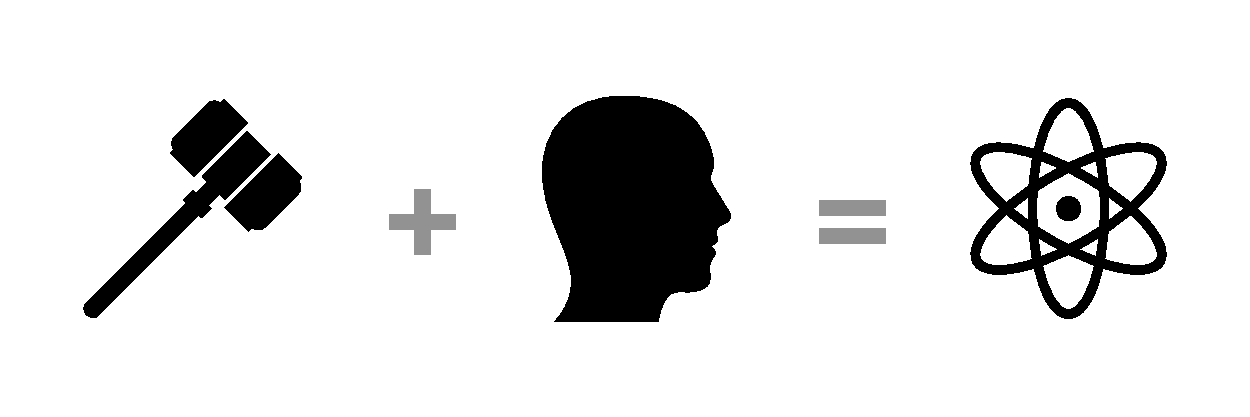
\includegraphics[width=0.5\textwidth]{wisdom.pdf}
\caption{Physically increasing wisdom.}
\label{fig:wisdom}
\end{figure}

Aenean venenatis metus eu odio dapibus sollicitudin faucibus sit amet nunc. Suspendisse a posuere massa. Suspendisse mollis ut ipsum et sodales.

\subsection{Morbi a pretium odio}
Curabitur placerat dapibus quam pretium suscipit. Proin pharetra vulputate eleifend. Curabitur molestie sapien a erat euismod pharetra. Nunc ante lectus, porttitor nec facilisis non, vestibulum ac ligula. Praesent at euismod nulla.

%auto-ignore
\section{Experiments}
\label{sec:experiment}

Lorem ipsum dolor sit amet, consectetur adipiscing elit. Nunc rhoncus libero sed fermentum semper. Ut semper condimentum gravida. Integer lorem enim, feugiat vitae purus ac, dictum porttitor elit. Curabitur non elit ac velit volutpat congue. Nulla facilisi. Morbi a pretium odio. Maecenas leo metus, consequat nec augue nec, luctus molestie magna.

%auto-ignore
\section{Conclusion}
\label{sec:conclusion}

Lorem ipsum dolor sit amet, consectetur adipiscing elit. Nunc rhoncus libero sed fermentum semper. Ut semper condimentum gravida. Integer lorem enim, feugiat vitae purus ac, dictum porttitor elit. Curabitur non elit ac velit volutpat congue. Nulla facilisi. Morbi a pretium odio. Maecenas leo metus, consequat nec augue nec, luctus molestie magna.


% Bibliography
\bibliography{bibliography/related,bibliography/method}
\bibliographystyle{template/acl_natbib}

% Appendix
\appendix
%auto-ignore
\section{Appendices}
\label{sec:appendix}

%Appendices are material that can be read, and include lemmas, formulas, proofs, and tables that are not critical to the reading and understanding of the paper.

%auto-ignore
\section{Supplemental Material}
\label{sec:supplemental}

%Submissions may include non-readable supplementary material used in the work and described in the paper.
%Any accompanying software and/or data should include licenses and documentation of research review as appropriate.


\end{document}
